\documentclass[presentation,professionalfonts]{beamer}


\usepackage[utf8]{inputenc}
\usepackage[T1]{fontenc}
\usepackage{graphicx}
\usepackage[normalem]{ulem}
\usepackage{amsmath}
\usepackage{IEEEtrantools}
\usepackage{bm}
\usepackage{hyperref}
\tolerance=1000
\usepackage{algorithm}
\usepackage{algpseudocode}
\usepackage{tikz}
\usepackage{xspace}
\usepackage{booktabs}
\usepackage{listings}
\usepackage{appendixnumberbeamer}

\usepackage[
backend=biber,
style=numeric,
sortlocale=en_US,
url=false,
doi=true,
eprint=false,
giveninits=false,
maxbibnames=20,
maxnames=20,
maxcitenames=4
]{biblatex}
\addbibresource{templ.bib}

\usepackage{lmodern}
\usefonttheme[onlymath]{serif}

\setbeamercovered{highly dynamic}
\setbeamertemplate{caption}[numbered]
\setbeamertemplate{bibliography item}[text]
\usetheme{TUW}

\newcommand{\semname}{Scheduling Algorithms for Clusters, Distributed Systems, and Multi-core Nodes}
\newcommand{\semester}{SS 2018}

\institute[TU Wien]{Seminar ``\semname''\\\semester}
\titlegraphic{
\includegraphics[height=.7cm]{./logos/par-logo.pdf}\quad
\includegraphics[height=.7cm]{./logos/info-logo.pdf}}

% change this, of course
\date{\today}
\title[Scheduling Jobs with Max-Min Fairness]{Scheduling Jobs across Geo-Distributed Datacenters with Max-Min Fairness}
\author[Aleksandr Lisianoi]{Aleksandr Lisianoi}

\begin{document}

\maketitle


\begin{frame}{Seminar Talk's Main Sources}
  \begin{enumerate}
  \item \fullcite{Chen2017}
  \end{enumerate}
\end{frame}

\begin{frame}{Outline}
  % \tableofcontents[currentsection]
  \tableofcontents
\end{frame}

\section{Introduction}

\begin{frame}{Problem Description}
  \begin{block}{The Main Question}
    Given a \emph{large volume} of data stored in \emph{geographically distributed} datacenters, how to effectively run \emph{multiple} analytical jobs in a \emph{fair} fashion?
    \end{block}

  Things to consider:

  \begin{enumerate}
    \item Data locality
    \item Network bandwidth
  \end{enumerate}
\end{frame}

\begin{frame}{What is an Analytic Job?}

  A data analytic job usually consists of several consecutive stages, each of which consists of several parallel tasks.

  Examples:
  \begin{itemize}
  \item 2007 The New York Times https://open.blogs.nytimes.com/2007/11/01/self-service-prorated-super-computing-fun/
  \item 2017 Spotify https://labs.spotify.com/2017/10/16/big-data-processing-at-spotify-the-road-to-scio-part-1/
    Alternating Least Squares: if User x Score matrix is binary, then the author could parallelize efficiently with Spark
    Spotify operates a Hadoop cluster to over 2500 nodes and over 100 PBs of capacity running about 20,000 independent jobs per day.
    \end{itemize}

\end{frame}

\begin{frame}{Analytic Job: Formal Definition}
  \begin{IEEEeqnarray*}{llCl}
    \text{Datacenter: }                                     & \mathcal{D}   &=& \left\{1, 2, \dots, J\right\} \\
    \text{Datacenter capacity for \(j\in\mathcal{D}\): }    & \mathcal{A}   &=& \left\{a_1, a_2, \dots, a_J\right\} \\
    \text{Data parallel job: }                              & \mathcal{K}   &=& \left\{1, 2, \dots, K\right\} \\
    \text{Parallel tasks for job \(k \in \mathcal{K}\): }   & \mathcal{T}_k &=& \left\{1, 2, \dots, n_k\right\} \\
  \end{IEEEeqnarray*}
  For each task \(i\in\mathcal{T}_k\) of job \(k\): network transfer time \(c^k_{i, j}\) and execution time \(e^k_{i, j}\) if datacenter \(j\) is used. Source datacenters for task \(i\) of job \(k\) are \(S^k_i\).

  \begin{equation*}
    c^k_{i, j} = \left\{ \,
    \begin{IEEEeqnarraybox}[][c]{l?s}
      \IEEEstrut
      0, &  when \(S^k_i = \left\{j\right\}\)\\
      \max_{s\in S^k_i, s\neq j}\left(\frac{d^{k, s}_i}{b_{s,j}}\right) & otherwise
      \IEEEstrut
    \end{IEEEeqnarraybox}
    \right.
  \end{equation*}
\end{frame}

\begin{frame}{Analytic Job: Formal Definition (continued)}
  \begin{IEEEeqnarray}{lrCll}
    \text{lexmin}_{\bm{x}} & \bm{f} &=&\left(\tau_1, \tau_2, \dots, \tau_K\right) &\\
    \text{s.t.} & \tau_k &=& \max_{i\in\mathcal{T}_k, j\in\mathcal{D}} x^k_{i, j}\left(c^k_{i, j} + e^k_{i, j}\right), &\forall k\in\mathcal{K} \label{eq:goal}\\
    &&& \sum_{k\in\mathcal{K}}\sum_{i\in\mathcal{T}_k} x^k_{i, j} \leq a_j, &\forall j\in\mathcal{D} \label{eq:capacity}\\
    &&& \sum_{j\in\mathcal{D}}x^k_{i, j} = 1, &\forall i\in\mathcal{T}_k, \forall k\in\mathcal{K} \label{eq:presence}\\
    &&& x^k_{i, j} \in \left\{0, 1\right\}. &\forall i \in \mathcal{T}_k, \forall j\in\mathcal{D}, \forall k\in\mathcal{K} \label{eq:onehot}
  \end{IEEEeqnarray}

  Constraint \eqref{eq:goal}: a task requires as long as its longest job. \\
  Constraint \eqref{eq:capacity}: capacity of the datacenter is not exceeded. \\
  Constraint \eqref{eq:presence}: each job is assigned to exactly one datacenter. \\
\end{frame}

\begin{frame}{Problem Transformations}
  From multiple-objective to single-objective optimization:
  \begin{IEEEeqnarray}{ll}
    \min_{\bm{x}} & \quad \max_{k\in\mathcal{K}}\left(\tau_k\right) \\
    \text{s.t.}  & \quad \text{Constraints \eqref{eq:goal}, \eqref{eq:capacity}, \eqref{eq:presence} and \eqref{eq:onehot} hold}
  \end{IEEEeqnarray}

  From non-linear constraints to linear constraints:

  \begin{IEEEeqnarray}{ll}
    \min_{\bm{x}} & \quad \max_{k\in\mathcal{K}}\left(\max_{i\in\mathcal{T}_k, j\in\mathcal{D}} x^k_{i, j}\left(c^k_{i, j} + e^k_{i, j}\right)\right) \\
    \text{s.t.}  & \quad \text{Constraints \eqref{eq:capacity}, \eqref{eq:presence} and \eqref{eq:onehot} hold}
    \end{IEEEeqnarray}
\end{frame}

\section{Experimental Evaluation}

\begin{frame}
  \frametitle{Experimental Results}
  \begin{center}
  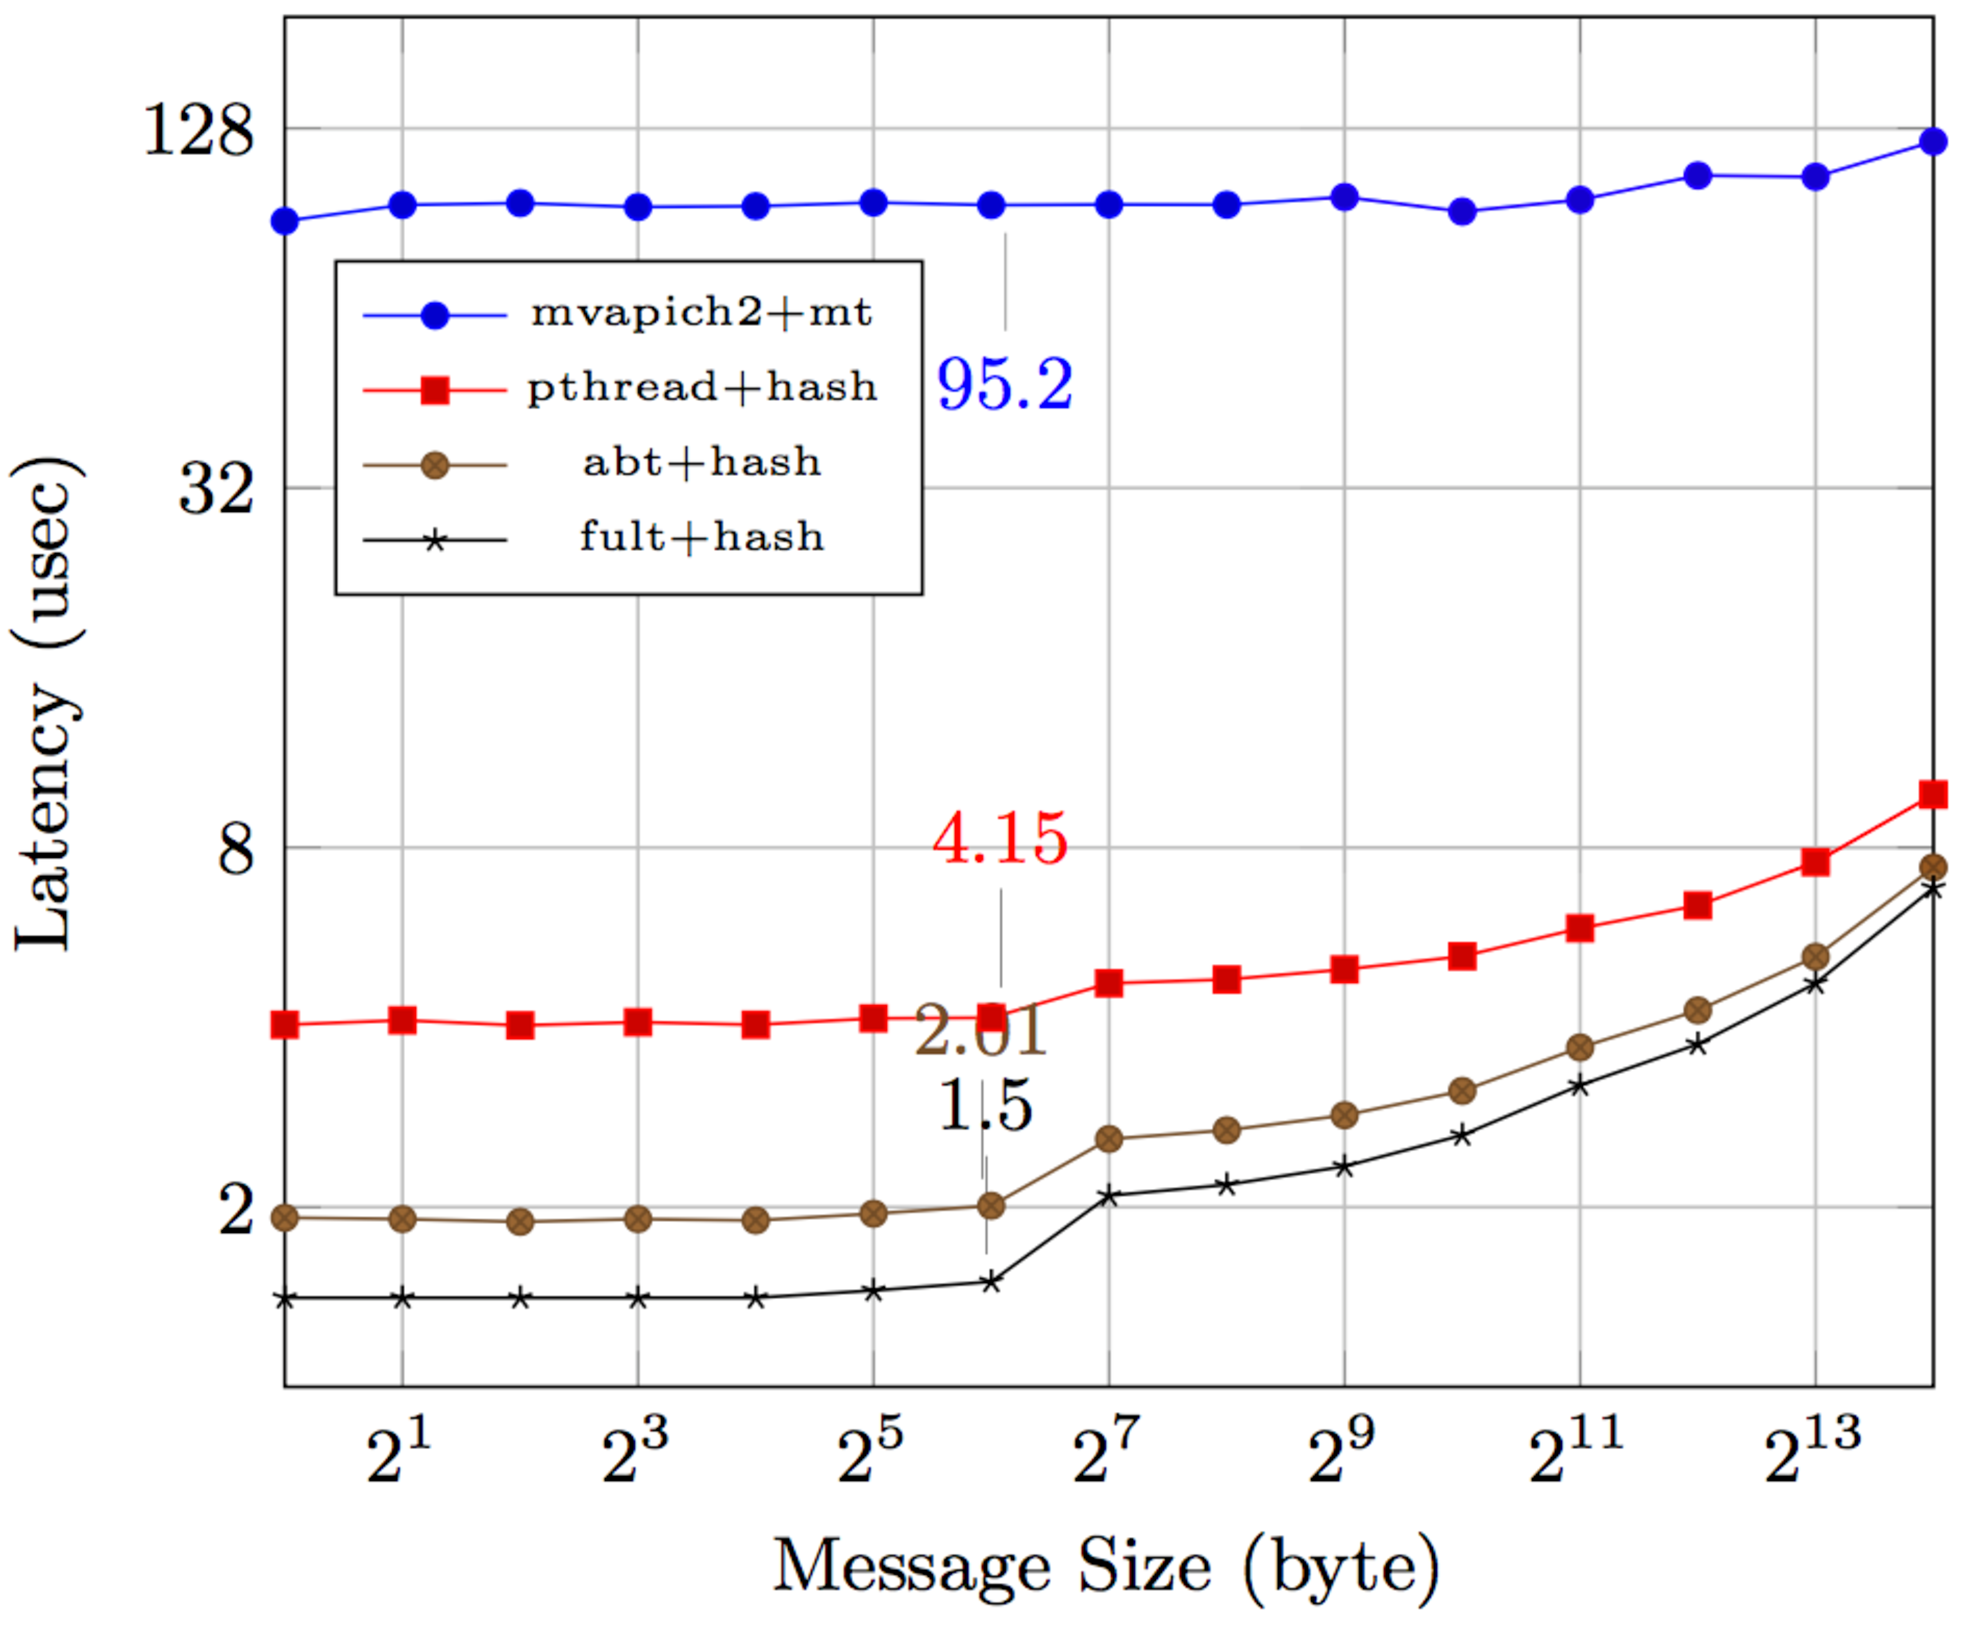
\includegraphics[width=.7\textwidth]{./graph1}\\
  image source: \textcite{Dang16}
  \end{center}
\end{frame}

\section{Conclusions}

\begin{frame}
  \frametitle{Conclusions}
  \begin{itemize}
  \item nice paper 
  \item substantial improvement
  \end{itemize}  
\end{frame}


\begin{frame}[fragile]{References}
\printbibliography
\end{frame}

\appendix

\begin{frame}{In Case You Expect Questions}
\centering
\begin{itemize}
\item foo
\item bar
\item barfoo
\end{itemize}
\end{frame}

\end{document}
